\documentclass[11pt,a4paper]{article}

% ---------- Packages ----------
\usepackage[utf8]{inputenc}
\usepackage[T1]{fontenc}
\usepackage[margin=1in]{geometry}
\usepackage[hidelinks]{hyperref}
\usepackage{graphicx}
\usepackage{booktabs}
\usepackage{array}
\usepackage{tabularx}
\usepackage{enumitem}
\usepackage{xcolor}
\usepackage{caption}
\captionsetup{format=plain,justification=raggedright,singlelinecheck=false}
\usepackage{listings}
\usepackage{float}            % [H] exact placement
\usepackage[section]{placeins}% keep floats in section
\usepackage{url}              % \path, \url (safe underscores + wrapping)
\usepackage{amsmath,amssymb,mathtools}
\usepackage{siunitx}
\usepackage{tikz}
\usetikzlibrary{arrows.meta,calc,decorations.pathreplacing}
\usepackage{seqsplit}         % break long identifiers if needed

% Improve line-breaking / avoid overfull boxes a bit
\emergencystretch=3em

% ---------- Listings (code + pseudocode) ----------
\lstdefinestyle{code}{
  basicstyle=\ttfamily\small,
  columns=fullflexible,
  frame=single,
  breaklines=true,
  showstringspaces=false,
  tabsize=2,
  upquote=true
}
\lstdefinelanguage{XML}{
  morestring=[b]",
  morecomment=[s]{<!--}{-->},
  morekeywords={xmlns,version,type}
}
\lstdefinelanguage{pseudo}{
  morekeywords={function,procedure,requires,ensures,for,while,if,else,elseif,return,break,continue,end,foreach,not,and,or},
  sensitive=true,
  morecomment=[l]{//}
}
\lstset{style=code}

% ---------- Math helpers ----------
\DeclareMathOperator{\smoothstep}{smoothstep}
\newcommand{\vect}[1]{\mathbf{#1}}
\newcommand{\unitvect}[1]{\hat{\mathbf{#1}}}

% Safer inline code for long tokens
\newcommand{\codepath}[1]{\path{#1}}            % breaks at / _ .
\newcommand{\codeid}[1]{\texttt{\seqsplit{#1}}} % breaks inside long identifiers

% ---------- Title ----------
\title{ARGoS Wind / Air Resistance — Developer Guide}
\author{Roi Sela}
\date{October 2025}

\begin{document}
\maketitle

\begin{center}
\small Repository: \href{https://github.com/roiSela/epcuk2}{project link}
\end{center}

\tableofcontents

\section*{Audience \& Scope}
This guide targets developers who will extend, maintain, or embed the project's wind / air-resistance behavior in ARGoS~3 (dynamics2d / Chipmunk engine). It covers architecture, the impulse pipeline, aerodynamic blocking via RAB, configuration schema, and extension points. Language-agnostic pseudocode is provided for core functions.

\section{Repository Overview}
\begin{tabularx}{\textwidth}{@{}p{.45\textwidth}X@{}}
\toprule
Path & Purpose \\
\midrule
\codepath{controllers/air_resistance} & Base controller (\texttt{CAirResistance}): wind + drive impulse pipeline, RAB-based aerodynamic blocking. \\
\codepath{controllers/wind_aware} & Example derived controller (behavior details are documented in the user manual). \\
\codepath{loop_functions/wind_loop_functions} & Logic-only loop functions to read wind from XML and expose it. \\
\codepath{loop_functions/wind_loop_functions (Qt)} & Qt user functions that draw the wind vector arrow in the world view. \\
\codepath{examples/} & Minimal runnable ARGoS configs (documented in the user manual). \\
\bottomrule
\end{tabularx}

\section{Architecture}
\subsection{Core Controller: \texttt{CAirResistance}}
\paragraph{Lifecycle and Extensibility.}
\texttt{CAirResistance} derives from \texttt{CCI\_Controller}. Lifecycle methods are virtual and designed for subclassing.

\paragraph{Important protected hooks (what they do).}
\begin{itemize}[leftmargin=*,itemsep=4pt]
  \item \textbf{\texttt{EnsurePhysicsHandle()}} — Idempotently cache the Chipmunk body (pointer, mass, space, COM) and derive the robot's effective radius in meters from the AABB. Safe to call every tick.
  \item \textbf{\texttt{GetYawRadians()}} — Return yaw \(\psi\) (world frame) from the positioning sensor; used for the forward unit vector \(\unitvect{f}(\psi)\).
  \item \textbf{\texttt{HandleAerodynamicsPreStep()}} — Reset \(\vect{J}_{\mathrm{sum}}\); add the wind impulse using the current effective wind \(\vect{w}_{\mathrm{eff}}\); broadcast the RAB radius (mm). No post-step scheduling here.
  \item \textbf{\texttt{HandleAerodynamicsPostStep()}} — Register a Chipmunk post-step callback to apply \(\vect{J}_{\mathrm{sum}}\) after collisions.
  \item \textbf{\texttt{ComputeEffectiveWind()}} — Compute and return \(\vect{w}_{\mathrm{eff}}=(1-r)\vect{w}\) where \(r\) is the wake reduction computed from neighbors (see Sec.~\ref{sec:wake-blocking}).
  \item \textbf{\texttt{IsBlockedByRAB(Real\& r)}} — From RAB neighbors, compute \(r\in[0,1]\) via geometric overlap of wakes (details in Sec.~\ref{sec:wake-blocking}).
  \item \textbf{\texttt{DriveImpulse(Real v\_cm\_s)}} — Add forward impulse \(\frac{m}{100}v\,\unitvect{f}(\psi)\) (cm/s \(\rightarrow\) m/s factor 1/100).
  \item \textbf{\texttt{ApplyWindImpulse()}} — Add \(\frac{m}{100}\,\vect{w}_{\mathrm{eff}}\) to the per-tick accumulator.
\end{itemize}

\paragraph{Impulse Pipeline (per tick).}
\begin{enumerate}[leftmargin=*,itemsep=2pt]
  \item \textbf{Pre-step}: Reset the impulse accumulator; compute and add the wind impulse (possibly reduced by blocking); broadcast radius via RAB.
  \item \textbf{Drive}: Add a forward drive impulse along current yaw using the desired base speed.
  \item \textbf{Post-step}: Schedule a single Chipmunk \emph{post-step} callback to apply the summed impulse after collisions.
\end{enumerate}

\paragraph{Physics Integration.}
We downcast the ARGoS \texttt{dynamics2d} model to either \codeid{CDynamics2DSingleBodyObjectModel} (e-puck2) or \codeid{CDynamics2DMultiBodyObjectModel} (foot-bot). For multi-body robots, body index~0 is treated as the chassis. AABB is used to derive a reasonable self-radius \(R\) (meters), clamped to sane limits.

\section{Configuration Interface (recap)}
Under \verb|<configuration>| declare:
\begin{lstlisting}[language=XML]
<air_resistance angle_deg="0" magnitude="15.0"/>
\end{lstlisting}
\(\texttt{angle\_deg}\) is the global wind direction (degrees, world frame); \(\texttt{magnitude}\) is wind speed in \si{cm/s}.  
Each controller instance accepts:
\begin{lstlisting}[language=XML]
<params velocity="15.0"/>
\end{lstlisting}

\section{Algorithmic Details (with Equations)}
\subsection{Impulse Model (first definition of \texorpdfstring{\(\vect{w}_{\mathrm{eff}}\)}{weff} + numeric example)}
Per tick we accumulate world-frame impulses:
\begin{align}
  \vect{J}_\text{wind}  &= \frac{m}{100}\,\underbrace{\vect{w}_\text{eff}}_{\text{effective wind in \si{cm/s}}},\\
  \vect{J}_\text{drive} &= \frac{m}{100}\,v_d\,\unitvect{f}(\psi),\\
  \vect{J}_\text{sum}   &= \vect{J}_\text{wind} + \vect{J}_\text{drive}.
\end{align}
\textbf{Definition.} Let \(\vect{w}\) be the global wind and \(r\in[0,1]\) the reduction due to upwind neighbors. The effective wind is
\[
  \boxed{\ \vect{w}_\text{eff} = (1-r)\,\vect{w}\ } \quad \text{(with \(r\) computed in Sec.~\ref{sec:wake-blocking}).}
\]
Here \(m\) is body mass (Chipmunk), \(v_d\) the desired forward speed (\si{cm/s}), and \(\unitvect{f}(\psi)\) the unit forward vector given yaw \(\psi\).
A single post-step callback applies \(\vect{J}_\text{sum}\) at the COM after collisions.

\paragraph{Numeric example (with picture).}
Let \(m=\SI{0.08}{kg}\), \(v_d=\SI{10}{cm/s}\), and \(\vect{w}=(\SI{20}{cm/s},0)\).  
If \(r=0.4\Rightarrow \vect{w}_\text{eff}=(\SI{12}{cm/s},0)\).  
With yaw \(\psi=60^\circ\), \(\unitvect{f}(\psi)=(\cos 60^\circ,\sin 60^\circ)=(0.5,0.866)\).
\[
\vect{J}_\text{wind}=\tfrac{0.08}{100}(12,0)=(0.0096,0),\quad
\vect{J}_\text{drive}=\tfrac{0.08}{100}\cdot10\,(0.5,0.866)=(0.0040,0.00693),
\]
so \(\boxed{\vect{J}_\text{sum}\approx(0.0136,\;0.00693)\ \mathrm{kg\,m/s}}\).

% --------- Your illustration: do not change ----------
% Figure 1: Visual impulse composition with step-by-step breakdown
\begin{figure}[H]
  \centering
  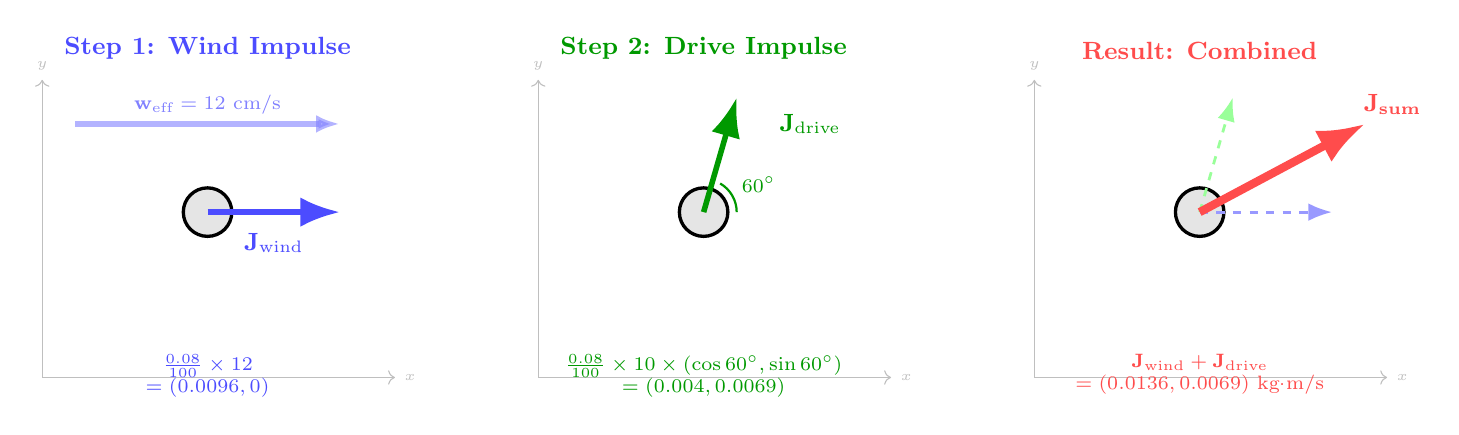
\begin{tikzpicture}[scale=1.4]
    % ===== STEP 1: Wind Component (LEFT) =====
    \begin{scope}[xshift=0cm]
      \node[above,font=\small\bfseries,blue!70] at (1.5,2.8) {Step 1: Wind Impulse};
      \filldraw[fill=gray!20,draw=black,very thick] (1.5,1.5) circle (0.22);
      \draw[->,gray!50] (0,0) -- (3.2,0) node[right,font=\tiny]{$x$};
      \draw[->,gray!50] (0,0) -- (0,2.7) node[above,font=\tiny]{$y$};
      \draw[-{Latex[length=3mm]},blue!50,line width=2pt,opacity=0.6] (0.3,2.3) -- (2.7,2.3);
      \node[above,blue!50,font=\scriptsize] at (1.5,2.3) {$\vect{w}_\text{eff}=12$ cm/s};
      \draw[-{Latex[length=5mm]},blue!70,line width=2pt] (1.5,1.5) -- (2.7,1.5);
      \node[below,blue!70,font=\small] at (2.1,1.4) {$\vect{J}_\text{wind}$};
      \node[below,blue!70,font=\scriptsize,align=center] at (1.5,0.3) {$\frac{0.08}{100}\times 12$\\$=(0.0096, 0)$};
    \end{scope}
    % ===== STEP 2: Drive Component (MIDDLE) =====
    \begin{scope}[xshift=4.5cm]
      \node[above,font=\small\bfseries,green!60!black] at (1.5,2.8) {Step 2: Drive Impulse};
      \filldraw[fill=gray!20,draw=black,very thick] (1.5,1.5) circle (0.22);
      \draw[->,gray!50] (0,0) -- (3.2,0) node[right,font=\tiny]{$x$};
      \draw[->,gray!50] (0,0) -- (0,2.7) node[above,font=\tiny]{$y$};
      \draw[green!60!black,thick] (1.8,1.5) arc[start angle=0,end angle=60,radius=0.3];
      \node[green!60!black,font=\scriptsize] at (2.0,1.75) {$60^\circ$};
      \draw[-{Latex[length=5mm]},green!60!black,line width=2pt] (1.5,1.5) -- ({1.5+0.6*cos(60)},{1.5+1.2*sin(60)});
      \node[right,green!60!black,font=\small] at (2.1,2.3) {$\vect{J}_\text{drive}$};
      \node[below,green!60!black,font=\scriptsize,align=center] at (1.5,0.3) {$\frac{0.08}{100}\times 10 \times (\cos 60^\circ, \sin 60^\circ)$\\$=(0.004, 0.0069)$};
    \end{scope}
    % ===== STEP 3: Combined Result (RIGHT) =====
    \begin{scope}[xshift=9cm]
      \node[above,font=\small\bfseries,red!70] at (1.5,2.8) {Result: Combined};
      \filldraw[fill=gray!20,draw=black,very thick] (1.5,1.5) circle (0.22);
      \draw[->,gray!50] (0,0) -- (3.2,0) node[right,font=\tiny]{$x$};
      \draw[->,gray!50] (0,0) -- (0,2.7) node[above,font=\tiny]{$y$};
      \draw[-{Latex[length=3mm]},blue!40,line width=1pt,dashed] (1.5,1.5) -- (2.7,1.5);
      \draw[-{Latex[length=3mm]},green!40,line width=1pt,dashed] (1.5,1.5) -- ({1.5+0.6*cos(60)},{1.5+1.2*sin(60)});
      \draw[-{Latex[length=6mm]},red!70,line width=3pt] (1.5,1.5) -- (3.0,2.3);
      \node[above right,red!70,font=\small\bfseries] at (2.9,2.3) {$\vect{J}_\text{sum}$};
      \node[below,red!70,font=\scriptsize,align=center] at (1.5,0.3) {$\vect{J}_\text{wind} + \vect{J}_\text{drive}$\\$=(0.0136, 0.0069)$ kg·m/s};
    \end{scope}
  \end{tikzpicture}
  \caption{Impulse composition example with $m=0.08$ kg, $v_d=10$ cm/s, $\vect{w}_\text{eff}=12$ cm/s, and $\psi=60^\circ$. \textbf{Left:} Wind pushes horizontally. \textbf{Middle:} Robot drives at $60^\circ$. \textbf{Right:} Both impulses combine (vector addition) to produce the actual motion impulse applied to the robot.}
\end{figure}
% ----------------------------------------------------

\subsection{Wake Blocking Reduction}
\label{sec:wake-blocking}

\paragraph{Problem we are solving.}
We need the shielding effect from an upwind blocker to fade out \emph{smoothly} with downwind distance. If we used a hard cutoff (on/off at some distance), tiny sensor noise or sub-tick motion would make the effect flicker: one tick ``blocked'', next tick ``not blocked''. That produces visible jerks and unstable dynamics. A smooth ramp avoids this.

For each upwind neighbor \(i\), compute an overlap score
\begin{equation}
  r_i = \exp\!\left(-\tfrac{1}{2}\left(\tfrac{\ell_\perp}{\sigma_\perp}\right)^2\right)
        \cdot \smoothstep\!\bigl(0, L;\, \ell_\parallel - g \bigr),
  \label{eq:ri}
\end{equation}
and take the boosted, clamped maximum
\[
  \boxed{\,r = \mathrm{clamp}\!\left(0,1,\;\gamma\cdot\max_{i\in\mathcal{N}} r_i\right)\,},\qquad
  \vect{w}_\text{eff}=(1-r)\vect{w}.
\]
Here \(\mathcal{N}\) is the set of upwind neighbors; \(\max_i\) means the \emph{maximum over neighbors}.

\paragraph{What is \(\smoothstep{}\) (and why use it)?}
\(\smoothstep(a,b;x)\) maps \(x\) from \([a,b]\) to a smooth ramp in \([0,1]\):
\[
\smoothstep(a,b;x)=
\begin{cases}
0 & x\le a,\\[2pt]
3t^2-2t^3 & a<x<b,\ \ t=\dfrac{x-a}{b-a},\\[6pt]
1 & x\ge b.
\end{cases}
\]
Its slope is zero at both ends, so the blocking grows and dies out gently instead of snapping on and off. In our case we apply it to \(\ell_\parallel-g\) over the interval \([0,L]\), which means: once the follower is a bit downwind of the blocker (past the upwind gate \(g\)), the reduction ramps in smoothly and reaches full effect by distance \(L\).

\paragraph{Parameter meanings (visualized in Fig.~\ref{fig:blocking_geometry} below).}
\begin{itemize}[leftmargin=*,itemsep=2pt]
  \item \(\ell_\parallel\): along-wind separation, i.e., the projection of the blocker\(\rightarrow\)follower vector onto the wind direction; it is the \emph{downwind distance from the blocker to the follower} (positive when the follower is downwind).
  \item \(\ell_\perp\): lateral offset from the wind centerline between the two robots.
  \item \(R\): robot radius in meters, derived from the AABB of the embodied entity (see Sec.~3); used as the base length scale.
  \item \(\sigma_\perp = \texttt{lateral\_reach\_radii}\cdot R\): lateral ``width'' of the wake (controls the Gaussian term).
  \item \(L = \texttt{shadow\_length\_radii}\cdot R\): downwind ``length'' of the wake (the smoothstep interval).
  \item \(g = \texttt{upwind\_gate\_radii}\cdot R\): small upwind gap to ignore near side-by-side cases before the ramp begins.
  \item \(\gamma=\texttt{gamma\_boost}\): optional emphasis of mid-range overlaps before clamping to \([0,1]\).
\end{itemize}

% --------- Your wake-geometry illustration: unchanged ----------
\begin{figure}[H]
  \centering
  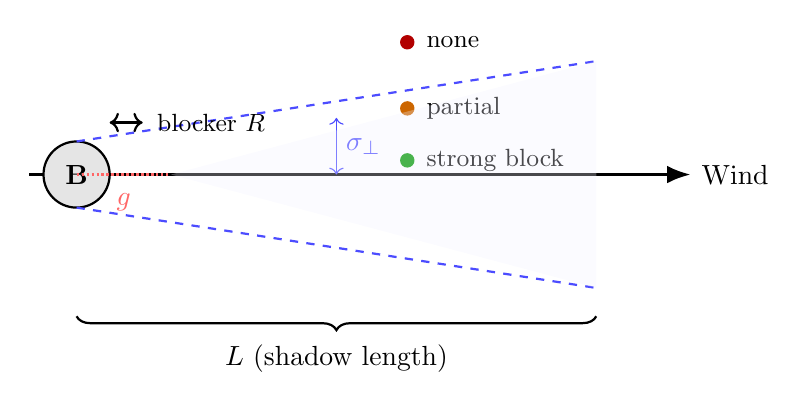
\begin{tikzpicture}[scale=1.2]
    % (unchanged figure from user)
    \draw[-{Latex[length=3mm]}, very thick] (-0.5,0) -- (6.5,0) node[right]{Wind};
    \draw[thick, fill=gray!20] (0,0) circle (0.35);
    \node at (0,0) {\textbf{B}};
    \draw[thick, densely dotted, red!60] (0,0) -- (1.0,0);
    \node[below, red!60] at (0.5,-0.1) {$g$};
    \draw[dashed, blue!70, thick] (0,0.35) -- (5.5,1.2);
    \draw[dashed, blue!70, thick] (0,-0.35) -- (5.5,-1.2);
    \draw[<->, blue!70] (2.75,0) -- (2.75,0.6);
    \node[right, blue!70] at (2.75,0.3) {$\sigma_\perp$};
    \draw[decorate, decoration={brace, amplitude=5pt, mirror}, thick] (0,-1.5) -- (5.5,-1.5);
    \node[below] at (2.75,-1.7) {$L$ (shadow length)};
    \filldraw[green!60!black] (3.5,0.15) circle (2pt);
    \node[right, font=\small] at (3.6,0.15) {strong block};
    \filldraw[orange!80!black] (3.5,0.7) circle (2pt);
    \node[right, font=\small] at (3.6,0.7) {partial};
    \filldraw[red!70!black] (3.5,1.4) circle (2pt);
    \node[right, font=\small] at (3.6,1.4) {none};
    \draw[thick, <->] (0.35,0.55) -- (0.7,0.55);
    \node[right, font=\small] at (0.75,0.55) {blocker $R$};
    \fill[blue!5, opacity=0.3] (1.0,0) -- (5.5,1.2) -- (5.5,-1.2) -- cycle;
  \end{tikzpicture}
  \caption{Blocking geometry. Adjusting $\sigma_\perp$ (lateral reach), $L$ (shadow length), $g$ (upwind gate), and $\gamma$ (boost) reshapes the wake and the final reduction $r$.}
  \label{fig:blocking_geometry}
\end{figure}
% ---------------------------------------------------------------

\paragraph{Two-blocker illustration (max over neighbors).}
% (Your two-blocker figure kept exactly)
\begin{figure}[H]
  \centering
  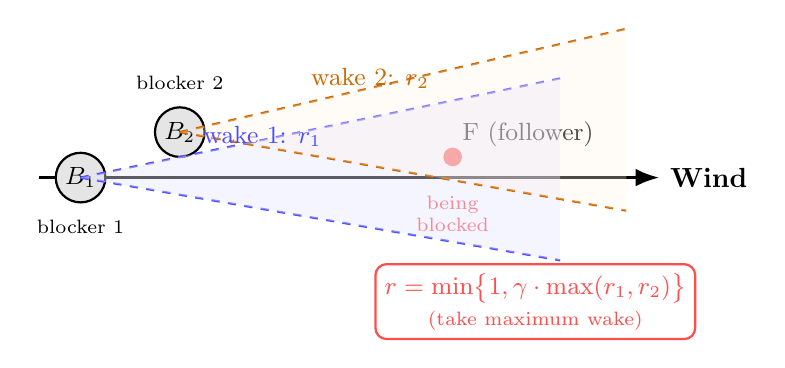
\begin{tikzpicture}[scale=1.05]
    % Wind axis
    \draw[-{Latex[length=3mm]},very thick] (-0.5,0) -- (7.0,0) node[right,font=\bfseries]{Wind};
    
    % Blocker 1 (lower left)
    \draw[thick, fill=gray!20] (0,0) circle (0.3); 
    \node at (0,0) {\small $B_1$};
    \node[below,font=\scriptsize] at (0,-0.4) {blocker 1};
    
    % Blocker 2 (upper, slightly right)
    \draw[thick, fill=gray!20] (1.2,0.55) circle (0.3); 
    \node at (1.2,0.55) {\small $B_2$};
    \node[above,font=\scriptsize] at (1.2,0.95) {blocker 2};
    
    % Follower F (the robot being blocked)
    \filldraw[red!70] (4.5,0.25) circle (3pt); 
    \node[above right,font=\small] at (4.5,0.25) {F (follower)};
    \node[below,red!70,font=\scriptsize,align=center] at (4.5,-0.1) {being\\blocked};
    
    % Wake boundaries for B1 (blue dashed)
    \draw[dashed, blue!70, thick] (0,0) -- (5.8,1.2);
    \draw[dashed, blue!70, thick] (0,0) -- (5.8,-1.0);
    \fill[blue!10, opacity=0.4] (0,0) -- (5.8,1.2) -- (5.8,-1.0) -- cycle;
    
    % Wake boundaries for B2 (orange dashed)
    \draw[dashed, orange!80!black, thick] (1.2,0.55) -- (6.6,1.8);
    \draw[dashed, orange!80!black, thick] (1.2,0.55) -- (6.6,-0.4);
    \fill[orange!10, opacity=0.3] (1.2,0.55) -- (6.6,1.8) -- (6.6,-0.4) -- cycle;
    
    % Labels for r_i values (wake regions)
    \node[blue!70,font=\small] at (2.2,0.5) {wake 1: $r_1$};
    \node[orange!80!black,font=\small] at (3.5,1.2) {wake 2: $r_2$};
    
    % Final formula (larger box)
    \node[red!70,font=\small,align=center,draw=red!70,fill=white,rounded corners,thick] 
      at (5.5,-1.5) {$r=\min\bigl\{1,\gamma\cdot\max(r_1,r_2)\bigr\}$\\
      \scriptsize (take maximum wake)};
  \end{tikzpicture}
  \caption{Two upwind blockers ($B_1$ and $B_2$) create overlapping wakes. The follower robot F experiences blocking from both. Each blocker produces $r_i$ via \eqref{eq:ri}. The final reduction $r$ is the boosted/clamped \emph{maximum} over all neighbor wakes\textemdash{}meaning F gets blocked by whichever wake is strongest at its position.}
\end{figure}

\section{Pseudocode: Core Functions}
Variables mirror the C++ but remain language-agnostic. Distances in meters unless noted; speeds in \si{cm/s}. Comments use only ASCII to avoid listing-encoding issues.

\subsection{\texttt{Init(t\_node)}}
\begin{lstlisting}[language=pseudo]
function Init(node)
  // devices
  rab_act  <- GetActuator("range_and_bearing")
  rab_sen  <- GetSensor  ("range_and_bearing")
  pos_sen  <- GetSensor  ("positioning")
  wheels   <- GetActuator("differential_steering")

  // controller params
  v_desired_cm_s <- ReadParam(node, "velocity", default=10.0)

  // wind from <configuration><air_resistance .../>
  (angle_deg, magnitude_cm_s) <- ReadGlobalWind()
  wind_cm_s <- (magnitude_cm_s * cos(rad(angle_deg)),
                magnitude_cm_s * sin(rad(angle_deg)))
end
\end{lstlisting}

\subsection{\texttt{EnsurePhysicsHandle()}}
\begin{lstlisting}[language=pseudo]
function EnsurePhysicsHandle()
  if body_ready: return

  // fetch entity + embodied component
  entity    <- GetSelfEntity()
  embodied  <- entity.GetComponent("body")

  // derive self radius from AABB (meters), clamp to sane range
  bb    <- embodied.GetBoundingBox()
  width <- bb.MaxCorner.x - bb.MinCorner.x
  depth <- bb.MaxCorner.y - bb.MinCorner.y
  self_radius_m <- 0.5 * max(width, depth)
  self_radius_m <- Clamp(self_radius_m, 0.01, 0.50)

  // cache dyn2d body + mass etc.
  model <- GetDynamics2DModelForRobot()
  if model is SingleBody: body <- model.GetBody()
  else:                   body <- model.GetBody(index=0)  // chassis
  mass_kg <- Chipmunk.GetMass(body)

  body_ready <- true
end
\end{lstlisting}

\subsection{\texttt{HandleAerodynamicsPreStep()}}
\begin{lstlisting}[language=pseudo]
function HandleAerodynamicsPreStep()
  EnsurePhysicsHandle()

  // reset per-tick accumulator
  J_sum <- (0, 0)

  // wind contribution using effective wind (Sec. 4.1, 4.2)
  ApplyWindImpulse()

  // RAB broadcast: radius in millimeters (byte 0 only)
  if rab_act != null:
      r_mm <- Clamp(round(self_radius_m * 1000), 0, 255)
      rab_act.SetData(0, r_mm)
end
\end{lstlisting}

\subsection{\texttt{ComputeEffectiveWind()}}
\begin{lstlisting}[language=pseudo]
function ComputeEffectiveWind()
  if Norm(wind_cm_s) < 1e-9: return wind_cm_s
  r <- 0.0
  if IsBlockedByRAB(out r):   // r computed by wake model (see Sec. 4.2)
      return max(0, 1 - r) * wind_cm_s
  else:
      return wind_cm_s
end
\end{lstlisting}

\subsection{\texttt{IsBlockedByRAB(out r)}}
\begin{lstlisting}[language=pseudo]
function IsBlockedByRAB(out r)
  r <- 0.0
  if pos_sen == null or rab_sen == null: return false
  if Norm(wind_cm_s) < 1e-9:             return false

  // Tunables (geometry in "blocker radii")
  lateral_reach_radii <- 3.0    // controls lateral Gaussian width
  shadow_length_radii <- 4.0    // how far wake reaches downwind
  gamma_boost         <- 2.0    // 1.0 disables boost
  upwind_gate_radii   <- 0.5    // minimum along-wind gap

  // World-frame unit wind direction
  wind_dir_hat <- Normalize(wind_cm_s)

  // My yaw (world), used to rotate RAB bearings
  yaw_world <- GetYawRadians()

  any <- false
  for msg in rab_sen.GetReadings():

      // range in cm -> meters
      range_m <- 0.01 * msg.Range
      if range_m <= 1e-6: continue

      // blocker radius from advertised byte[0] (mm->m) else fallback
      blocker_r_m <- self_radius_m
      if Size(msg.Data) >= 1:
          adv_m <- 0.001 * msg.Data[0]
          if 0.005 < adv_m and adv_m < 0.20: blocker_r_m <- adv_m

      // bearing to neighbor in world frame
      bearing_world <- yaw_world + msg.HorizontalBearing

      // vector ME->OTHER and OTHER->ME (meters, world)
      me_to_other <- (range_m * cos(bearing_world),
                      range_m * sin(bearing_world))
      other_to_me <- -me_to_other

      // along-wind component (positive means neighbor is upwind)
      along_m <- Dot(other_to_me, wind_dir_hat)

      // upwind gate: require some min gap to avoid side-by-side cases
      gate_m <- max(1e-6, upwind_gate_radii * blocker_r_m)
      if along_m <= gate_m: continue

      // lateral offset from wind centerline
      lateral_vec <- other_to_me - along_m * wind_dir_hat
      lateral_m   <- Norm(lateral_vec)

      // wake widths and fades (Sec. 4.2)
      sigma <- lateral_reach_radii * blocker_r_m
      L     <- shadow_length_radii * blocker_r_m

      lateral_cov <- exp(-0.5 * (lateral_m / max(1e-6, sigma))^2)
      fade        <- smoothstep(0, L, along_m - gate_m)
      red_i       <- lateral_cov * fade

      // optional non-linear emphasis
      red_i <- 1 - (1 - red_i) ^ gamma_boost

      r   <- max(r, red_i)   // max over neighbors
      any <- true

  r <- min(1.0, r)
  return any and (r > 1e-6)
end
\end{lstlisting}

\subsection{\texttt{DriveImpulse(v\_cm\_s)}}
\begin{lstlisting}[language=pseudo]
function DriveImpulse(v_cm_s)
  yaw <- GetYawRadians()
  fwd <- (cos(yaw), sin(yaw))              // unit vector, world frame
  J_sum += (mass_kg/100.0) * v_cm_s * fwd
end
\end{lstlisting}

\subsection{\texttt{ApplyWindImpulse()}}
\begin{lstlisting}[language=pseudo]
function ApplyWindImpulse()
  w_eff_cm_s <- ComputeEffectiveWind()
  if Norm(w_eff_cm_s) < 1e-9: return
  J_sum += (mass_kg/100.0) * w_eff_cm_s
end
\end{lstlisting}

\subsection{\texttt{HandleAerodynamicsPostStep()}}
\begin{lstlisting}[language=pseudo]
function HandleAerodynamicsPostStep()
  space <- Chipmunk.Space(body)
  Chipmunk.AddPostStepCallback(space, lambda:
      Chipmunk.ApplyImpulseAtWorldPoint(body, J_sum, position=COM))
end
\end{lstlisting}

\subsection{\texttt{GetYawRadians()}}
\begin{lstlisting}[language=pseudo]
function GetYawRadians()
  q <- pos_sen.GetReading().Orientation()
  return q.Yaw()
end
\end{lstlisting}

\section{Tuning and Debugging}
\subsection*{Key tunables (typical defaults)}
\begin{itemize}[leftmargin=*,itemsep=2pt]
  \item \(\texttt{lateral\_reach\_radii}\) widens or narrows the Gaussian cross-section. Larger \(\Rightarrow\) stronger blocking even with lateral offset.
  \item \(\texttt{shadow\_length\_radii}\) lengthens the downwind extent. Larger \(\Rightarrow\) blocking persists farther downwind.
  \item \(\texttt{upwind\_gate\_radii}\) ignores near side-by-side neighbors (requires some minimum along-wind separation).
  \item \(\texttt{gamma\_boost}\) emphasizes mid-range overlaps (\(r \leftarrow \min(1,\gamma\cdot r)\)).
\end{itemize}

\subsection*{Debug tips}
\begin{itemize}[leftmargin=*,itemsep=2pt]
  \item Print intermediate terms inside the blocking loop: \(\ell_\parallel\), \(\ell_\perp\), \(r_i\), and the final \(r\).
  \item Verify the on-screen wind arrow matches your XML.
  \item If a robot seems unaffected, check: advertised radius byte (mm) \(\rightarrow\) meters, AABB-derived \(R\), and that neighbors are truly upwind (positive \(\ell_\parallel\)).
\end{itemize}

\section*{Appendix: Minimal C++ touchpoints (orientation only)}
\subsection*{Post-step application (Chipmunk)}
\begin{lstlisting}[language=C++]
cpSpaceAddPostStepCallback(space, ApplyAccumPostStep, m_ptBody, payload);
\end{lstlisting}

\subsection*{RAB radius broadcast (mm)}
\begin{lstlisting}[language=C++]
UInt8 r_mm = (UInt8) std::min(255.0, std::round(m_fSelfRadiusM * 1000.0));
m_pcRABAct->SetData(0, r_mm);
\end{lstlisting}

\section*{References}
\begin{thebibliography}{1}
\bibitem{StolfiDanoy2023}
D.~H. Stolfi and G.~Danoy, ``Design and analysis of an E-Puck2 robot
plug-in for the ARGoS simulator,'' \emph{Robotics and Autonomous Systems},
vol.~164, p.~104412, 2023. doi: \href{https://doi.org/10.1016/j.robot.2023.104412}{10.1016/j.robot.2023.104412}.
\end{thebibliography}

\end{document}
